\documentclass[aspectratio=169]{beamer}

% ── Theme ────────────────────────────────────────────────────────────────────
\usetheme{Madrid}
\usecolortheme{seahorse}
\usefonttheme{professionalfonts}

% ── Packages ─────────────────────────────────────────────────────────────────
\usepackage{listings}       % code listings
\usepackage{xcolor}         % colours
\usepackage{tikz}           % diagrams
\usepackage{booktabs}       % nice tables
\usepackage{hyperref}
\usepackage{textcomp}
\usepackage{microtype}

% ── Listing style ─────────────────────────────────────────────────────────────
\definecolor{codebg}{HTML}{1E1E2E}
\definecolor{codegreen}{HTML}{A6E3A1}
\definecolor{codeblue}{HTML}{89DCEB}
\definecolor{codeyellow}{HTML}{F9E2AF}
\definecolor{codegray}{HTML}{6C7086}
\definecolor{codepurple}{HTML}{CBA6F7}
\definecolor{codeorange}{HTML}{FAB387}
\definecolor{codewhite}{HTML}{CDD6F4}
\definecolor{alertred}{HTML}{F38BA8}

\lstdefinestyle{asm}{
  backgroundcolor=\color{codebg},
  basicstyle=\ttfamily\footnotesize\color{codewhite},
  keywordstyle=\color{codepurple}\bfseries,
  commentstyle=\color{codegray}\itshape,
  stringstyle=\color{codegreen},
  numberstyle=\tiny\color{codegray},
  numbers=left, numbersep=6pt,
  breaklines=true, frame=single,
  rulecolor=\color{codepurple},
  morekeywords={BITS,ORG,global,extern,section,db,dw,dd,dq,times,equ,
                mov,xor,cli,sti,hlt,jmp,jc,jz,call,ret,int,push,pop,
                lodsb,test,lgdt,or,in,out,iret,
                ah,al,ax,bx,cx,dx,si,di,sp,bp,
                ds,es,fs,gs,ss,cs,
                eax,ebx,ecx,edx,esi,edi,esp,ebp,
                cr0,cr3,ENTRY,SECTIONS},
  tabsize=4
}

\lstdefinestyle{clang}{
  backgroundcolor=\color{codebg},
  basicstyle=\ttfamily\footnotesize\color{codewhite},
  keywordstyle=\color{codepurple}\bfseries,
  commentstyle=\color{codegray}\itshape,
  stringstyle=\color{codegreen},
  numberstyle=\tiny\color{codegray},
  numbers=left, numbersep=6pt,
  breaklines=true, frame=single,
  rulecolor=\color{codeblue},
  language=C,
  tabsize=4
}

\lstdefinestyle{makefile}{
  backgroundcolor=\color{codebg},
  basicstyle=\ttfamily\footnotesize\color{codewhite},
  keywordstyle=\color{codeyellow}\bfseries,
  commentstyle=\color{codegray}\itshape,
  numberstyle=\tiny\color{codegray},
  numbers=left, numbersep=6pt,
  breaklines=true, frame=single,
  rulecolor=\color{codeyellow},
  tabsize=4
}

\lstdefinestyle{linker}{
  backgroundcolor=\color{codebg},
  basicstyle=\ttfamily\footnotesize\color{codewhite},
  keywordstyle=\color{codeorange}\bfseries,
  commentstyle=\color{codegray}\itshape,
  numberstyle=\tiny\color{codegray},
  numbers=left, numbersep=6pt,
  breaklines=true, frame=single,
  rulecolor=\color{codeorange},
  tabsize=4
}

% ── Metadata ──────────────────────────────────────────────────────────────────
\title[Writing a Minimal x86 OS]{%
  \textbf{Writing a Minimal x86 Operating System}\\
  \small From BIOS Boot to Kernel in Protected Mode}
\subtitle{A Step-by-Step Guide for Beginners}
\author{MyOS Project}
\date{March 2026}
\institute{From scratch, in Assembly and C}

% ── Helper: coloured box ──────────────────────────────────────────────────────
\newcommand{\concept}[2]{%
  \begin{block}{#1}\smallskip #2\smallskip\end{block}\vspace{5pt}}

\newcommand{\warn}[1]{%
  \begin{alertblock}{Important}\smallskip #1\smallskip\end{alertblock}\vspace{5pt}}

% ─────────────────────────────────────────────────────────────────────────────
\begin{document}

% ── TITLE ─────────────────────────────────────────────────────────────────────
\begin{frame}
  \titlepage
\end{frame}

% ── TABLE OF CONTENTS ─────────────────────────────────────────────────────────
\begin{frame}{Table of Contents}
  \tableofcontents
\end{frame}

%% ════════════════════════════════════════════════════════════════════════════
\section{What is an Operating System?}
%% ════════════════════════════════════════════════════════════════════════════

\begin{frame}{What is an Operating System?}
  \begin{columns}[T]
    \column{0.55\textwidth}
    An \textbf{Operating System (OS)} is software that:
    \begin{itemize}
      \item Acts as a \textbf{bridge} between hardware and programs
      \item Manages \textbf{CPU time} (scheduling)
      \item Manages \textbf{RAM} (memory management)
      \item Manages \textbf{devices} (keyboard, disk, screen)
      \item Provides a \textbf{file system}
      \item Gives programs a safe, isolated environment
    \end{itemize}
    \vspace{6pt}
    \textit{Examples: Linux, Windows, macOS, FreeBSD}
    \column{0.42\textwidth}
    \vspace{8pt}
    \begin{center}
    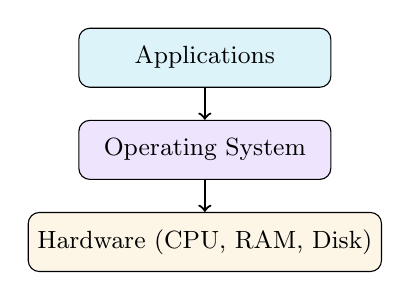
\begin{tikzpicture}[scale=0.9,
        box/.style={rectangle,draw,rounded corners,
                    minimum width=3.2cm,minimum height=0.75cm,
                    align=center,font=\small}]
      \node[box,fill=codeblue!30]  (app)  at (0,2.6) {Applications};
      \node[box,fill=codepurple!30](os)   at (0,1.3) {Operating System};
      \node[box,fill=codeyellow!30](hw)   at (0,0)   {Hardware (CPU, RAM, Disk)};
      \draw[->,thick] (app) -- (os);
      \draw[->,thick] (os)  -- (hw);
    \end{tikzpicture}
    \end{center}
  \end{columns}
\end{frame}

\begin{frame}{What We Are Building}
  We will build the \textbf{smallest possible OS}:
  \begin{itemize}
    \item A \textbf{bootloader} -- loads the kernel from disk
    \item A \textbf{kernel} -- runs in 32-bit Protected Mode, prints to screen
    \item \textbf{No files, no processes, no system calls} -- just raw hardware access
  \end{itemize}
  \vspace{8pt}
  \concept{Why do this?}{
    Writing an OS from scratch teaches you more about computers than any other project. You learn exactly what happens when you press the power button.
  }
\end{frame}

%% ════════════════════════════════════════════════════════════════════════════
\section{How a Computer Boots}
%% ════════════════════════════════════════════════════════════════════════════

\begin{frame}{The Boot Process --- Overview}
  \begin{center}
  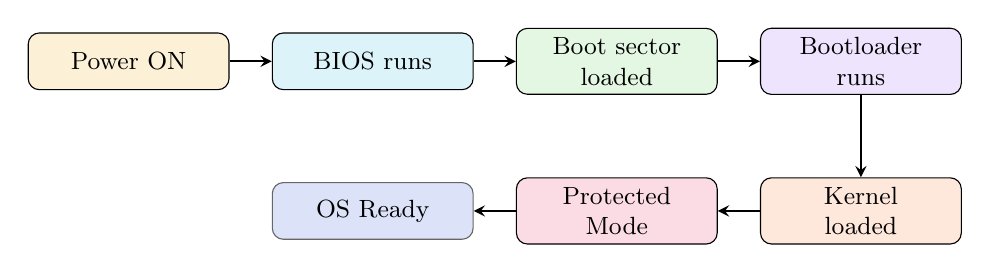
\begin{tikzpicture}[
      box/.style={rectangle,draw,rounded corners=4pt,
                  minimum width=2.55cm,minimum height=0.72cm,
                  align=center,font=\small},
      arr/.style={->,thick,>=stealth}]
    %% ── Row 1: left → right ──────────────────────────────────
    \node[box,fill=codeyellow!50]  (power) at (0,   0)   {Power ON};
    \node[box,fill=codeblue!30]    (bios)  at (3.1, 0)   {BIOS runs};
    \node[box,fill=codegreen!30]   (mbr)   at (6.2, 0)   {Boot sector\\loaded};
    \node[box,fill=codepurple!30]  (boot)  at (9.3, 0)   {Bootloader\\runs};
    %% ── Row 2: right → left (snake) ─────────────────────────
    \node[box,fill=codeorange!30]  (kern)  at (9.3,-1.9) {Kernel\\loaded};
    \node[box,fill=alertred!30]    (pm)    at (6.2,-1.9) {Protected\\Mode};
    \node[box,fill=codewhite!70,draw=black!60] (os) at (3.1,-1.9) {OS Ready};
    %% ── Arrows row 1 ─────────────────────────────────────────
    \draw[arr] (power)--(bios);
    \draw[arr] (bios)--(mbr);
    \draw[arr] (mbr)--(boot);
    %% ── Snake connector (straight down) ─────────────────────
    \draw[arr] (boot)--(kern);
    %% ── Arrows row 2 ─────────────────────────────────────────
    \draw[arr] (kern)--(pm);
    \draw[arr] (pm)--(os);
  \end{tikzpicture}
  \end{center}
  \vspace{4pt}
  Each arrow is a distinct phase. We write code for \textbf{every phase}.
\end{frame}

\begin{frame}{Step 1 -- BIOS (Basic Input/Output System)}
  \begin{columns}[T]
    \column{0.55\textwidth}
    \vspace{4pt}
    \begin{itemize}
      \item Firmware \textbf{burned into a chip} on the motherboard
      \item First thing CPU runs when powered on
      \item Runs a \textbf{Power-On Self Test (POST)}
      \item Finds a bootable disk, reads its \textbf{first 512 bytes}
      \item Loads those 512 bytes to address \texttt{0x7C00} in RAM
      \item Checks bytes 511--512 = \texttt{0x55 0xAA} (magic number)
      \item Jumps to \texttt{0x7C00} -- your code runs!
    \end{itemize}
    \column{0.42\textwidth}
    \vspace{4pt}
    \begin{center}
    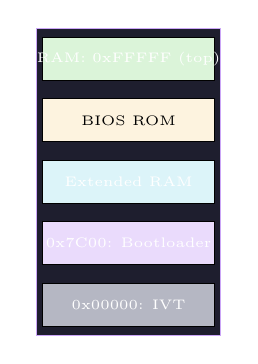
\begin{tikzpicture}[scale=0.78]
      \draw[fill=codebg,draw=codepurple] (0,0) rectangle (3,5);
      \draw[fill=codegreen!40]  (0.1,4.15) rectangle (2.9,4.85); \node[font=\tiny,white] at (1.5,4.5) {RAM: 0xFFFFF (top)};
      \draw[fill=codeyellow!40] (0.1,3.15) rectangle (2.9,3.85); \node[font=\tiny] at (1.5,3.5) {BIOS ROM};
      \draw[fill=codeblue!30]   (0.1,2.15) rectangle (2.9,2.85); \node[font=\tiny,white] at (1.5,2.5) {Extended RAM};
      \draw[fill=codepurple!40] (0.1,1.15) rectangle (2.9,1.85); \node[font=\tiny,white] at (1.5,1.5) {0x7C00: Bootloader};
      \draw[fill=codegray!50]   (0.1,0.15) rectangle (2.9,0.85); \node[font=\tiny,white] at (1.5,0.5) {0x00000: IVT};
    \end{tikzpicture}
    \end{center}
  \end{columns}
\end{frame}

\begin{frame}{Step 2 -- The Boot Sector (MBR)}
  \concept{Master Boot Record (MBR)}{
    The very first sector (512 bytes) of a bootable disk. The BIOS reads it into RAM at \texttt{0x7C00} and transfers control to it.
  }
  \begin{columns}[T]
    \column{0.5\textwidth}
    \vspace{2pt}
    \textbf{512-byte layout:}
    \begin{itemize}
      \item Bytes 0--509: Your bootloader code
      \item Bytes 510--511: \texttt{0x55 0xAA} (boot signature)
    \end{itemize}
    \vspace{8pt}
    \warn{If the last two bytes are NOT \texttt{0x55AA}, the BIOS ignores the disk entirely!}
    \column{0.47\textwidth}
    \vspace{6pt}
    \begin{center}
    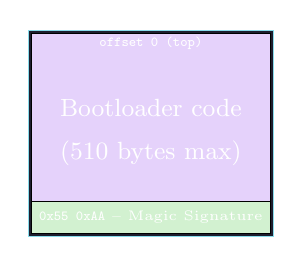
\begin{tikzpicture}[scale=0.82]
      \draw[fill=codebg,draw=codeblue] (0,0) rectangle (3.8,3.2);
      \draw[fill=codepurple!50] (0.05,0.55) rectangle (3.75,3.15);
      \draw[fill=codegreen!50]  (0.05,0.05) rectangle (3.75,0.55);
      \node[font=\small,white] at (1.9,2.0) {Bootloader code};
      \node[font=\small,white] at (1.9,1.3) {(510 bytes max)};
      \node[font=\tiny,white]  at (1.9,0.3){\texttt{0x55 0xAA} -- Magic Signature};
      \node[font=\tiny,white]  at (1.9,3.0){\texttt{offset 0 (top)}};
    \end{tikzpicture}
    \end{center}
  \end{columns}
\end{frame}

%% ════════════════════════════════════════════════════════════════════════════
\section{CPU Modes Explained}
%% ════════════════════════════════════════════════════════════════════════════

\begin{frame}{CPU Modes: Real Mode vs Protected Mode}
  \begin{columns}[T]
    \column{0.54\textwidth}
    \begin{tabular}{lll}
      \toprule
      & \textbf{Real Mode} & \textbf{Protected}\\
      \midrule
      Bits        & 16-bit           & 32-bit\\
      Max RAM     & 1 MB             & 4 GB\\
      Safety      & None             & Segments + paging\\
      BIOS calls  & Yes (\texttt{int})& No\\
      Used by     & Bootloader       & Kernel / OS\\
      \bottomrule
    \end{tabular}
    \column{0.43\textwidth}
    \concept{Real Mode}{
      CPU starts here on boot. 8086 compatibility mode. BIOS services available. Only 1\,MB RAM accessible.
    }
    \concept{Protected Mode}{
      Full 32-bit power. Memory protection enforced. No BIOS. You own the hardware.
    }
  \end{columns}
\end{frame}

\begin{frame}{Memory Addressing in Real Mode}
  In real mode the CPU uses \textbf{segment:offset} addressing:
  \[
    \text{Physical Address} = \text{Segment} \times 16 + \text{Offset}
  \]
  \begin{exampleblock}{Example}
    \texttt{ES = 0x0000}, \texttt{BX = 0x1000} $\Rightarrow$ physical address = \texttt{0x0000 * 16 + 0x1000 = 0x1000}
  \end{exampleblock}
  \vspace{4pt}
  \begin{itemize}
    \item \texttt{CS:IP} = Code Segment : Instruction Pointer (where CPU fetches code)
    \item \texttt{SS:SP} = Stack Segment : Stack Pointer
    \item \texttt{DS:SI} = Data Segment : Source Index (string ops)
    \item \texttt{ES:BX} = Extra Segment : Base register (disk read destination)
  \end{itemize}
\end{frame}

\begin{frame}{x86 Registers Cheat Sheet}
  \begin{columns}
    \column{0.48\textwidth}
    \textbf{16-bit general purpose:}\\[4pt]
    \begin{tabular}{ll}
      \texttt{AX} & Accumulator (results)\\
      \texttt{BX} & Base (memory addresses)\\
      \texttt{CX} & Counter (loops)\\
      \texttt{DX} & Data (I/O ports)\\
      \texttt{SI} & Source Index\\
      \texttt{DI} & Destination Index\\
      \texttt{SP} & Stack Pointer\\
      \texttt{BP} & Base Pointer (stack frame)\\
    \end{tabular}
    \column{0.48\textwidth}
    \textbf{In 32-bit mode, prefix with E:}\\[4pt]
    \texttt{EAX, EBX, ECX, EDX, ESI, EDI, ESP, EBP}\\[8pt]
    \textbf{Segment registers:}\\[4pt]
    \begin{tabular}{ll}
      \texttt{CS} & Code Segment\\
      \texttt{DS} & Data Segment\\
      \texttt{SS} & Stack Segment\\
      \texttt{ES,FS,GS} & Extra segments\\
    \end{tabular}
  \end{columns}
\end{frame}

%% ════════════════════════════════════════════════════════════════════════════
\section{Tools and Project Structure}
%% ════════════════════════════════════════════════════════════════════════════

\begin{frame}{Tools We Use}
  \begin{tabular}{lll}
    \toprule
    \textbf{Tool} & \textbf{What it does} & \textbf{Install}\\
    \midrule
    \texttt{nasm}         & Assembles \texttt{.asm} to machine code     & \texttt{brew install nasm}\\
    \texttt{i686-elf-gcc} & Cross-compiles C for bare-metal x86         & \texttt{brew install i686-elf-gcc}\\
    \texttt{i686-elf-ld}  & Links object files using our linker script  & (bundled with above)\\
    \texttt{qemu-system-i386}& Emulates a 32-bit x86 PC               & \texttt{brew install qemu}\\
    \texttt{dd}           & Writes raw bytes to disk image              & built-in on macOS/Linux\\
    \bottomrule
  \end{tabular}
  \vspace{8pt}
  \concept{Why a cross-compiler?}{
    Your Mac runs ARM or x86-64. We need code for 32-bit x86. A \textbf{cross-compiler} runs on your machine but produces code for a \emph{different} target architecture.
  }
\end{frame}

\begin{frame}[fragile]{Project File Structure}
  \begin{columns}[T]
    \column{0.42\textwidth}
    \begin{exampleblock}{Directory layout}
\begin{verbatim}
myos/
├── boot/
│   └── bootloader.asm
├── kernel/
│   ├── kernel_entry.asm
│   ├── kernel.c
│   ├── screen.c
│   └── screen.h
├── linker.ld
└── Makefile
\end{verbatim}
    \end{exampleblock}
    \column{0.55\textwidth}
    \vspace{6pt}
    \begin{center}
    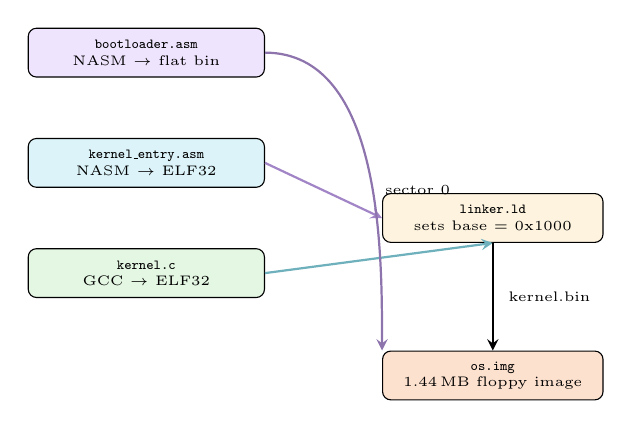
\begin{tikzpicture}[>=stealth,
        src/.style={rectangle,draw,rounded corners=3pt,
                    minimum width=3.0cm,minimum height=0.62cm,
                    align=center,font=\tiny},
        tgt/.style={rectangle,draw,rounded corners=3pt,
                    minimum width=2.8cm,minimum height=0.62cm,
                    align=center,font=\tiny}]
      %% ── Source files (left column, x=0) ──────────────────
      \node[src,fill=codepurple!30](bl) at(0, 3.2){\texttt{bootloader.asm}\\NASM $\to$ flat bin};
      \node[src,fill=codeblue!30]  (ka) at(0, 1.8){\texttt{kernel\_entry.asm}\\NASM $\to$ ELF32};
      \node[src,fill=codegreen!30] (kc) at(0, 0.4){\texttt{kernel.c}\\GCC $\to$ ELF32};
      %% ── Output files (right column, x=4.4) ───────────────
      \node[tgt,fill=codeyellow!40](ln) at(4.4, 1.1){\texttt{linker.ld}\\sets base = 0x1000};
      \node[tgt,fill=codeorange!40](img)at(4.4,-0.9){\texttt{os.img}\\1.44\,MB floppy image};
      %% ── Arrows: ELF objects → linker ─────────────────────
      \draw[->,thick,draw=codepurple!80!black] (ka.east)--(ln.west);
      \draw[->,thick,draw=codeblue!80!black]   (kc.east)--(ln.south);
      %% ── Arrow: linker → os.img (kernel.bin) ──────────────
      \draw[->,thick] (ln.south)--(img.north)
            node[midway,right=2pt,font=\tiny]{kernel.bin};
      %% ── Arrow: bootloader → os.img (sector 0) ────────────
      \draw[->,thick,draw=codepurple!70!black]
            (bl.east) .. controls +(1.5,0) and +(0,1.2) .. (img.north west)
            node[pos=0.6,above right,font=\tiny]{sector 0};
    \end{tikzpicture}
    \end{center}
  \end{columns}
\end{frame}

%% ════════════════════════════════════════════════════════════════════════════
\section{The Bootloader}
%% ════════════════════════════════════════════════════════════════════════════

\begin{frame}[fragile]{Bootloader --- Header and Segment Setup}
  \begin{lstlisting}[style=asm]
[BITS 16]       ; Tell NASM: generate 16-bit code
[ORG 0x7C00]    ; Tell NASM: code will be at 0x7C00 in RAM

start:
    ; DL = boot drive number passed by BIOS — save FIRST
    mov [boot_drive], dl

    cli             ; Disable interrupts during setup
    xor ax, ax      ; AX = 0  (xor with self = fastest way to zero)
    mov ds, ax      ; Data Segment = 0
    mov es, ax      ; Extra Segment = 0
    mov ss, ax      ; Stack Segment = 0
    mov sp, 0x7C00  ; Stack just below our code (grows downward)
    sti             ; Re-enable interrupts — needed for BIOS disk calls
  \end{lstlisting}
  \vspace{2pt}
  \begin{itemize}
    \small
    \item \texttt{[BITS 16]} / \texttt{[ORG ...]} are \textbf{NASM directives} — not CPU instructions
    \item \texttt{cli} / \texttt{sti} toggle the CPU interrupt flag
    \item \texttt{xor ax, ax} is faster than \texttt{mov ax, 0} (1 byte vs 3 bytes)
  \end{itemize}
\end{frame}

\begin{frame}[fragile]{Bootloader --- BIOS Disk Reset}
  \begin{lstlisting}[style=asm]
    ; Reset disk controller before reading
    ; AH=0 with int 0x13 = reset drive
    xor ah, ah
    mov dl, [boot_drive]   ; which drive to reset
    int 0x13               ; BIOS disk interrupt
    jc disk_error          ; CF (carry flag) set = error
  \end{lstlisting}
  \vspace{4pt}
  \concept{BIOS Interrupts (\texttt{int})}{
    In real mode, \texttt{int 0x13} calls the BIOS disk service. You pass arguments in registers and BIOS fills result registers. \texttt{AH} selects the function.
  }
  \vspace{4pt}
  \concept{The Carry Flag (CF)}{
    Many BIOS calls set the \textbf{Carry Flag} on error. \texttt{jc} = ``Jump if Carry'' -- this is how we detect failures without \texttt{errno}.
  }
\end{frame}

\begin{frame}[fragile]{Bootloader --- Loading the Kernel from Disk}
  \begin{lstlisting}[style=asm]
    ; BIOS int 0x13, AH=0x02 = Read Sector(s)
    xor ax, ax
    mov es, ax             ; ES = 0x0000
    mov bx, 0x1000         ; BX = 0x1000 -> destination = 0x0000:0x1000

    mov ah, 0x02           ; function: read sectors
    mov al, 16             ; read 16 sectors (16 x 512 = 8 KB)
    mov ch, 0              ; cylinder number = 0
    mov cl, 2              ; start sector = 2  (sector 1 = our bootloader)
    mov dh, 0              ; head number = 0
    mov dl, [boot_drive]   ; drive (0x00=floppy, 0x80=hard disk)
    int 0x13
    jc disk_error          ; CF set if read failed
  \end{lstlisting}
  \vspace{2pt}
  \small
  \begin{tabular}{ll}
    \texttt{ES:BX} target & physical = ES*16+BX = 0x0000*16+0x1000 = \textbf{0x1000}\\
    Sectors & 1-indexed; sector 1 = boot sector, sector 2 = first kernel byte\\
  \end{tabular}
\end{frame}

\begin{frame}[fragile]{Bootloader --- The A20 Line}
  \begin{lstlisting}[style=asm]
enable_a20:
    in  al, 0x92        ; read System Control Port A
    or  al, 0x02        ; set bit 1 = A20 enable
    out 0x92, al        ; write back
    ret
  \end{lstlisting}
  \vspace{6pt}
  \concept{What is A20?}{
    Old 8086 CPUs had 20 address lines (A0--A19) = 1 MB max. When 286 added line A20, BIOS \textbf{disabled it} by default for backward compatibility. We must \textbf{enable A20} before accessing memory above 1 MB. Without it, addresses above 1 MB wrap around silently.
  }
  \vspace{4pt}
  \texttt{in}/\texttt{out} = x86 instructions to read/write I/O ports (direct hardware register access).
\end{frame}

%% ════════════════════════════════════════════════════════════════════════════
\section{The GDT and Protected Mode Switch}
%% ════════════════════════════════════════════════════════════════════════════

\begin{frame}{The Global Descriptor Table (GDT)}
  In protected mode, memory is described by \textbf{segment descriptors} inside the GDT.
  \vspace{4pt}
  \begin{columns}[T]
    \column{0.52\textwidth}
    Each descriptor is \textbf{8 bytes} and describes:
    \begin{itemize}
      \item \textbf{Base} -- where the segment starts in RAM
      \item \textbf{Limit} -- how large the segment is
      \item \textbf{Access} -- read/write/execute permissions
      \item \textbf{Ring level} -- privilege (ring 0 = kernel)
    \end{itemize}
    \vspace{6pt}
    We need at minimum \textbf{3 descriptors}:
    \begin{enumerate}
      \item Null descriptor (required by CPU)
      \item Code segment descriptor
      \item Data segment descriptor
    \end{enumerate}
    \column{0.45\textwidth}
    \vspace{6pt}
    \begin{center}
    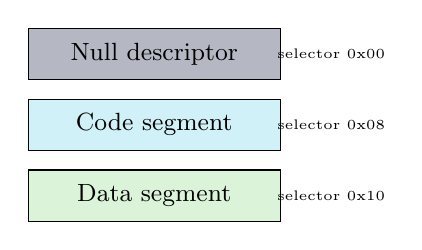
\begin{tikzpicture}[scale=0.9,
        box/.style={rectangle,draw,minimum width=3.2cm,
                    minimum height=0.65cm,align=center,font=\small}]
      \node[box,fill=codegray!50]   (n) at(0,2.0){Null descriptor};
      \node[box,fill=codeblue!40]   (c) at(0,1.0){Code segment};
      \node[box,fill=codegreen!40]  (d) at(0,0.0){Data segment};
      \node[font=\tiny,right] at(1.6,2.0){selector 0x00};
      \node[font=\tiny,right] at(1.6,1.0){selector 0x08};
      \node[font=\tiny,right] at(1.6,0.0){selector 0x10};
    \end{tikzpicture}
    \end{center}
    \vspace{6pt}
    \small Segment selector = GDT index $\times$ 8
  \end{columns}
\end{frame}

\begin{frame}[fragile]{GDT Code in Assembly}
  \begin{lstlisting}[style=asm]
gdt_start:
    dq 0                   ; Null descriptor (8 zero bytes — mandatory)

    ; Code segment: base=0, limit=4GB, 32-bit, ring 0, executable
    dw 0xFFFF              ; limit[15:0]  = 0xFFFF
    dw 0x0000              ; base[15:0]   = 0
    db 0x00                ; base[23:16]  = 0
    db 10011010b           ; Access byte  = present|ring0|code|exec|readable
    db 11001111b           ; Flags+limit  = 4K granularity|32-bit|limit[19:16]
    db 0x00                ; base[31:24]  = 0

    ; Data segment: same but not executable, writable
    dw 0xFFFF
    dw 0x0000
    db 0x00
    db 10010010b           ; Access byte  = present|ring0|data|writable
    db 11001111b
    db 0x00
gdt_end:

gdt_descriptor:
    dw gdt_end - gdt_start - 1   ; GDT size - 1 (limit)
    dd gdt_start                  ; 32-bit address of GDT
  \end{lstlisting}
\end{frame}

\begin{frame}[fragile]{Entering Protected Mode}
  \begin{lstlisting}[style=asm]
    cli                    ; MUST disable interrupts — no IDT exists yet!

    lgdt [gdt_descriptor]  ; Load GDT register with our table

    ; Set bit 0 of CR0 (Protection Enable bit)
    mov eax, cr0
    or  eax, 0x1
    mov cr0, eax

    ; Far jump: selector 0x08 (code segment) flushes CPU pipeline
    ; and fully completes the switch to protected mode
    jmp 0x08:pm_entry
  \end{lstlisting}
  \vspace{4pt}
  \warn{You MUST \texttt{cli} before switching! Any interrupt in PM without an IDT causes a \textbf{Triple Fault} → CPU resets → OS reboots. This causes the ``blinking'' bug.}
  \vspace{4pt}
  \concept{CR0 Register}{
    \textbf{Control Register 0} has special CPU flags. Bit 0 = Protection Enable. Setting it switches the CPU to protected mode. You cannot use general registers; you must use \texttt{EAX} and \texttt{cr0}.
  }
\end{frame}

\begin{frame}[fragile]{32-bit Protected Mode Entry}
  \begin{lstlisting}[style=asm]
[BITS 32]           ; Now NASM generates 32-bit code
pm_entry:
    ; Load data segment selector (0x10) into all data segment registers
    mov ax, 0x10
    mov ds, ax
    mov es, ax
    mov fs, ax
    mov gs, ax
    mov ss, ax

    mov esp, 0x90000  ; Set up stack at 0x90000 (safe area below 1 MB)

    jmp 0x1000        ; Jump to loaded kernel at physical address 0x1000
  \end{lstlisting}
  \vspace{4pt}
  \begin{itemize}
    \item We point every segment register at selector \texttt{0x10} (data descriptor)
    \item Both base=0, limit=4 GB → \textbf{flat memory model} (simplest)
    \item Stack grows \textbf{downward} from \texttt{0x90000}
  \end{itemize}
\end{frame}

\begin{frame}[fragile]{Bootloader --- Print Routine and Boot Signature}
  \begin{lstlisting}[style=asm]
print16:
    mov ah, 0x0E      ; BIOS teletype: print char in AL
.loop:
    lodsb             ; AL = byte at [DS:SI],  SI++
    test al, al       ; is AL zero? (null terminator)
    jz .done
    int 0x10          ; BIOS video interrupt: print AL
    jmp .loop
.done:
    ret

disk_error:
    mov si, msg_disk_err
    call print16
    hlt               ; Stop CPU

msg_boot     db "Booting MyOS...", 13, 10, 0  ; 13=CR, 10=LF
msg_disk_err db "Disk read error!", 13, 10, 0
boot_drive   db 0             ; 1-byte variable to store drive number

times 510 - ($ - $$) db 0    ; Pad remaining space with zeros
dw 0xAA55                     ; Boot signature (little-endian)
  \end{lstlisting}
  \vspace{2pt}
  \small \texttt{\$} = current address, \texttt{\$\$} = start of section. \texttt{510 - (\$ - \$\$)} = bytes remaining before signature.
\end{frame}

%% ════════════════════════════════════════════════════════════════════════════
\section{The Kernel Entry Point}
%% ════════════════════════════════════════════════════════════════════════════

\begin{frame}[fragile]{Kernel Entry --- Why Assembly First?}
  \concept{C needs a stack and a clean environment}{
    Before \texttt{kernel\_main()} can run, the CPU needs a stack pointer and correct segment registers. C assumes these exist! We set them up in a tiny assembly stub.
  }
  \vspace{6pt}
  \begin{lstlisting}[style=asm]
[BITS 32]            ; 32-bit protected mode code

global _start        ; Export _start so the linker can find it
extern kernel_main   ; kernel_main is defined in kernel.c

_start:
    mov esp, 0x90000   ; Stack pointer (already set by bootloader,
                       ; but we set it again for safety)
    call kernel_main   ; Call our C function

    ; If kernel_main ever returns, halt safely
    cli                ; Disable interrupts — no IDT exists
.hang:
    hlt                ; Halt CPU (low power state)
    jmp .hang          ; If NMI wakes us, halt again
  \end{lstlisting}
\end{frame}

\begin{frame}[fragile]{Why \texttt{global} and \texttt{extern}?}
  \begin{columns}[T]
    \column{0.5\textwidth}
    \vspace{2pt}
    \textbf{In kernel\_entry.asm:}
    \begin{lstlisting}[style=asm]
global _start     ; visible to linker
extern kernel_main ; defined elsewhere
    \end{lstlisting}
    \vspace{6pt}
    \textbf{In kernel.c:}
    \begin{lstlisting}[style=clang]
// Linker finds this as "kernel_main"
void kernel_main(void) {
    // ...
}
    \end{lstlisting}
    \column{0.47\textwidth}
    \vspace{2pt}
    \concept{Symbols and Linking}{
      A \textbf{symbol} is a name for an address. The \textbf{linker} connects symbols across object files. \texttt{global} exports; \texttt{extern} imports.
    }
    \begin{center}
    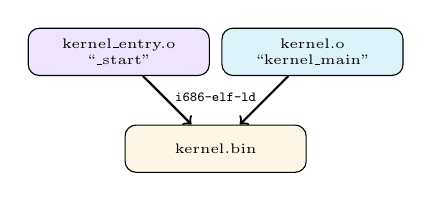
\begin{tikzpicture}[scale=0.82,
        box/.style={rectangle,draw,rounded corners,font=\tiny,
                    minimum width=2.3cm,minimum height=0.6cm,align=center}]
      \node[box,fill=codepurple!30](a) at(0,2.0){kernel\_entry.o\\``\_start''};
      \node[box,fill=codeblue!30]  (b) at(3.0,2.0){kernel.o\\``kernel\_main''};
      \node[box,fill=codeyellow!30](c) at(1.5,0.5){kernel.bin};
      \draw[->,thick](a)--(c);
      \draw[->,thick](b)--(c);
      \node[font=\tiny,align=center] at(1.5,1.3){\texttt{i686-elf-ld}};
    \end{tikzpicture}
    \end{center}
  \end{columns}
\end{frame}

%% ════════════════════════════════════════════════════════════════════════════
\section{The Linker Script}
%% ════════════════════════════════════════════════════════════════════════════

\begin{frame}[fragile]{The Linker Script Explained}
  \begin{lstlisting}[style=linker]
ENTRY(_start)          /* Tell linker: execution starts at _start */

SECTIONS
{
  . = 0x1000;          /* Load address: kernel lives at 0x1000 in RAM */

  .text : {            /* Code section */
    *(.text*)          /*   include .text from ALL object files */
  }

  .rodata : {          /* Read-only data (string literals etc.) */
    *(.rodata*)
  }

  .data : {            /* Initialised global variables */
    *(.data*)
  }

  .bss : {             /* Uninitialised globals (zero-filled) */
    *(.bss*)
    *(COMMON)
  }
}
  \end{lstlisting}
\end{frame}

\begin{frame}{Linker Script Concepts}
  \concept{Why no \texttt{[ORG]} in kernel ASM?}{
    \texttt{[ORG]} is only valid in NASM flat-binary mode. When compiling to ELF format, the \textbf{linker} sets addresses via \texttt{linker.ld}. Using \texttt{[ORG]} in an ELF object gives:
    \texttt{error: unrecognized directive}
  }
  \concept{. = 0x1000 (location counter)}{
    The dot \texttt{.} is the linker's current address counter. Setting \texttt{. = 0x1000} places all following sections at physical address \texttt{0x1000} --- exactly where the bootloader loaded the kernel.
  }
  \begin{tabular}{lll}
    \toprule
    \textbf{File type} & \textbf{Address control} & \textbf{Why}\\
    \midrule
    Bootloader (\texttt{-f bin}) & \texttt{[ORG 0x7C00]} & BIOS puts it there\\
    Kernel (\texttt{-f elf32}) & \texttt{linker.ld: . = 0x1000} & Bootloader loads it there\\
    \bottomrule
  \end{tabular}
\end{frame}

%% ════════════════════════════════════════════════════════════════════════════
\section{VGA Text Mode and the Kernel}
%% ════════════════════════════════════════════════════════════════════════════

\begin{frame}{VGA Text Mode --- Writing to the Screen}
  \concept{VGA Text Buffer at 0xB8000}{
    In text mode, the screen is a grid of \textbf{80 columns × 25 rows}. Each cell is \textbf{2 bytes}: one for the character (ASCII), one for colour. Writing to \texttt{0xB8000} instantly appears on screen -- no API needed!
  }
  \vspace{6pt}
  \begin{center}
  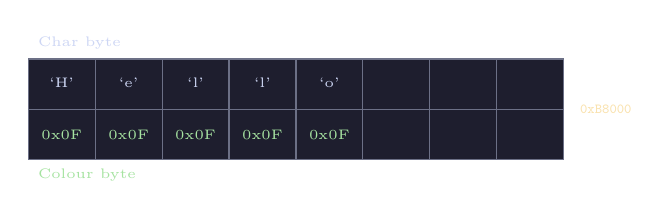
\begin{tikzpicture}[scale=0.85]
    \draw[fill=codebg,draw=codeblue] (0,0) rectangle (8,1.5);
    % char row
    \draw[draw=codegray](0,0.75)rectangle(1,1.5); \draw[draw=codegray](1,0.75)rectangle(2,1.5);
    \draw[draw=codegray](2,0.75)rectangle(3,1.5); \draw[draw=codegray](3,0.75)rectangle(4,1.5);
    \draw[draw=codegray](4,0.75)rectangle(5,1.5); \draw[draw=codegray](5,0.75)rectangle(6,1.5);
    \draw[draw=codegray](6,0.75)rectangle(7,1.5); \draw[draw=codegray](7,0.75)rectangle(8,1.5);
    % colour row
    \draw[draw=codegray](0,0)rectangle(1,0.75); \draw[draw=codegray](1,0)rectangle(2,0.75);
    \draw[draw=codegray](2,0)rectangle(3,0.75); \draw[draw=codegray](3,0)rectangle(4,0.75);
    \draw[draw=codegray](4,0)rectangle(5,0.75); \draw[draw=codegray](5,0)rectangle(6,0.75);
    \draw[draw=codegray](6,0)rectangle(7,0.75); \draw[draw=codegray](7,0)rectangle(8,0.75);
    \node[font=\tiny,color=codewhite] at (0.5,1.15){`H'};
    \node[font=\tiny,color=codewhite] at (1.5,1.15){`e'};
    \node[font=\tiny,color=codewhite] at (2.5,1.15){`l'};
    \node[font=\tiny,color=codewhite] at (3.5,1.15){`l'};
    \node[font=\tiny,color=codewhite] at (4.5,1.15){`o'};
    \node[font=\tiny,color=codegreen] at (0.5,0.37){0x0F};
    \node[font=\tiny,color=codegreen] at (1.5,0.37){0x0F};
    \node[font=\tiny,color=codegreen] at (2.5,0.37){0x0F};
    \node[font=\tiny,color=codegreen] at (3.5,0.37){0x0F};
    \node[font=\tiny,color=codegreen] at (4.5,0.37){0x0F};
    \node[font=\tiny,color=codewhite,above right] at(0,1.5){Char byte};
    \node[font=\tiny,color=codegreen,below right] at(0,0){Colour byte};
    \node[font=\tiny,right,color=codeyellow] at(8.1,0.75){\texttt{0xB8000}};
  \end{tikzpicture}
  \end{center}
  \vspace{4pt}
  \textbf{Index} for cell (row, col): \quad \texttt{index = row * 80 + col}\\
  \textbf{Full cell address}: \quad \texttt{0xB8000 + index * 2}
\end{frame}

\begin{frame}{VGA Colour Byte}
  The colour byte = \texttt{background << 4 | foreground}
  \vspace{4pt}
  \begin{tabular}{lll}
    \toprule
    Decimal & Hex & Colour\\
    \midrule
    0  & 0x0 & Black     \quad 8  = 0x8 Dark grey\\
    1  & 0x1 & Blue      \quad 9  = 0x9 Light blue\\
    2  & 0x2 & Green     \quad 10 = 0xA Light green\\
    3  & 0x3 & Cyan      \quad 11 = 0xB Light cyan\\
    4  & 0x4 & Red       \quad 12 = 0xC Light red\\
    5  & 0x5 & Magenta   \quad 13 = 0xD Light magenta\\
    6  & 0x6 & Brown     \quad 14 = 0xE Yellow\\
    7  & 0x7 & Light grey\quad 15 = 0xF White (bright)\\
    \bottomrule
  \end{tabular}
  \vspace{6pt}
  \begin{exampleblock}{Example}
    \texttt{0x0F} = background 0 (black) | foreground 15 (bright white)\\
    \texttt{0x0A} = background 0 (black) | foreground 10 (light green)
  \end{exampleblock}
\end{frame}

%% ════════════════════════════════════════════════════════════════════════════
\section{The Makefile and Build System}
%% ════════════════════════════════════════════════════════════════════════════

\begin{frame}[fragile]{The Makefile}
  \begin{lstlisting}[style=makefile]
AS      := nasm
LD      := i686-elf-ld
CC      := i686-elf-gcc
CFLAGS  := -m32 -ffreestanding -fno-pie -fno-stack-protector \
           -nostdlib -nostdinc -O2 -Wall -Wextra
LDFLAGS := -T linker.ld -nostdlib

$(BUILD)/boot.bin: boot/bootloader.asm
    $(AS) -f bin $< -o $@          # flat binary, no ELF wrapper

$(BUILD)/kernel_entry.o: kernel/kernel_entry.asm
    $(AS) -f elf32 $< -o $@        # ELF32 object file

$(BUILD)/kernel.o: kernel/kernel.c
    $(CC) $(CFLAGS) -c $< -o $@    # compile only, no link

$(BUILD)/screen.o: kernel/screen.c
  $(CC) $(CFLAGS) -c $< -o $@    # terminal driver object

$(BUILD)/kernel.bin: $(BUILD)/kernel_entry.o $(BUILD)/kernel.o $(BUILD)/screen.o
    $(LD) $(LDFLAGS) $^ --oformat binary -o $@
  \end{lstlisting}
\end{frame}

\begin{frame}[fragile]{Makefile --- Building the Disk Image}
  \begin{lstlisting}[style=makefile]
$(BUILD)/os.img: $(BUILD)/boot.bin $(BUILD)/kernel.bin
    # 1. Create blank 1.44 MB floppy image (2880 sectors x 512 bytes)
    dd if=/dev/zero of=$@ bs=512 count=2880 status=none

    # 2. Write bootloader at sector 0 (byte 0)
    dd if=$(BUILD)/boot.bin of=$@ conv=notrunc bs=512 seek=0 status=none

    # 3. Write kernel starting at sector 1 (byte 512)
    dd if=$(BUILD)/kernel.bin of=$@ conv=notrunc bs=512 seek=1 status=none

run: $(BUILD)/os.img
    qemu-system-i386 -fda $(BUILD)/os.img  # boot as floppy A:
  \end{lstlisting}
  \vspace{4pt}
  \concept{Why a 1.44 MB image?}{
    A plain \texttt{cat boot.bin kernel.bin} gives a 1355-byte file. BIOS trying to read 16 sectors past the end fails with a disk error. A proper floppy image has all sectors \textbf{pre-allocated as zeros}, so every sector is readable.
  }
\end{frame}

\begin{frame}{Compiler Flags Explained}
  \begin{tabular}{ll}
    \toprule
    \textbf{Flag} & \textbf{Meaning}\\
    \midrule
    \texttt{-m32}                & Emit 32-bit x86 code\\
    \texttt{-ffreestanding}      & No standard library, no OS assumed\\
    \texttt{-fno-pie}            & No Position-Independent Executable (fixed addresses)\\
    \texttt{-fno-stack-protector}& No stack canaries (needs libc to initialise)\\
    \texttt{-nostdlib}           & Don't link standard library (\texttt{libc})\\
    \texttt{-nostdinc}           & Don't include standard headers\\
    \texttt{-O2}                 & Optimisation level 2\\
    \texttt{-Wall -Wextra}       & All warnings enabled\\
    \texttt{-c}                  & Compile only (produce \texttt{.o}), don't link\\
    \bottomrule
  \end{tabular}
  \vspace{6pt}
  Without \texttt{-ffreestanding -nostdlib}, GCC would try to link \texttt{main()}, \texttt{\_start} from \texttt{libc}, \texttt{printf}, etc. -- none of which exist in our OS.
\end{frame}

%% ════════════════════════════════════════════════════════════════════════════
\section{Common Bugs and How We Fixed Them}
%% ════════════════════════════════════════════════════════════════════════════

\begin{frame}[fragile]{Bug \#1 --- \texttt{[ORG]} in ELF File}
  \begin{alertblock}{Error}
    \texttt{error: unrecognised directive [ORG]}
  \end{alertblock}
  \vspace{6pt}
  \begin{columns}[T]
    \column{0.48\textwidth}
    \textbf{Wrong:}
    \begin{lstlisting}[style=asm]
; kernel_entry.asm
[ORG 0x1000]   ; BAD for ELF!
[BITS 16]
_start:
    call kernel_main
    jmp $
    \end{lstlisting}
    \column{0.48\textwidth}
    \textbf{Fixed:}
    \begin{lstlisting}[style=asm]
; kernel_entry.asm
[BITS 32]       ; 32-bit PM code
global _start   ; export to linker
extern kernel_main
_start:
    mov esp, 0x90000
    call kernel_main
    cli
.hang: hlt
    jmp .hang
    \end{lstlisting}
  \end{columns}
  \vspace{4pt}
  Address is set in \texttt{linker.ld} with \texttt{. = 0x1000} instead.
\end{frame}

\begin{frame}{Bug \#2 --- Disk Read Error}
  \begin{alertblock}{Symptom}
    BIOS prints ``Disk read error!'' immediately after ``Booting MyOS\ldots''
  \end{alertblock}
  \vspace{4pt}
  \textbf{Three causes, all fixed:}
  \begin{enumerate}
    \item \textbf{Image too small} --- \texttt{cat} gave a 1355-byte file; sectors 2--17 didn't exist.\\
      \textit{Fix: Use \texttt{dd} to create a full 1.44 MB image first.}
    \item \textbf{Boot drive number lost} --- \texttt{DL} (drive number) was overwritten before \texttt{int 0x13}.\\
      \textit{Fix: Save \texttt{DL} to memory on entry: \texttt{mov [boot\_drive], dl}}
    \item \textbf{No disk reset} --- Dirty controller state from BIOS.\\
      \textit{Fix: Call \texttt{int 0x13 / AH=0} (reset) before reading.}
  \end{enumerate}
\end{frame}

\begin{frame}{Bug \#3 --- OS Blinking / Rapid Restart Loop}
  \begin{alertblock}{Symptom}
    QEMU flickers between ``Booting MyOS\ldots'' and MyOS screen rapidly.
  \end{alertblock}
  \vspace{6pt}
  \concept{The Triple Fault Cycle}{
    \begin{enumerate}
      \item Kernel loads and runs (displays screen)
      \item An interrupt fires (BIOS timer, NMI, etc.)
      \item No IDT set up $\Rightarrow$ CPU raises a \textbf{Double Fault}
      \item No double-fault handler $\Rightarrow$ CPU raises a \textbf{Triple Fault}
      \item Triple fault = CPU \textbf{resets} $\Rightarrow$ BIOS runs again $\Rightarrow$ repeat
    \end{enumerate}
  }
  \vspace{4pt}
  \textbf{Fixes:}
  \begin{itemize}
    \item \texttt{cli} before \texttt{lgdt} + \texttt{CR0} switch (never re-enabled)
    \item Kernel idle: \texttt{cli} then \texttt{hlt} loop (not \texttt{for(;;)\{\}})
  \end{itemize}
\end{frame}

%% ════════════════════════════════════════════════════════════════════════════
\section{Full Memory Map}
%% ════════════════════════════════════════════════════════════════════════════

\begin{frame}{x86 Memory Map (Low 1 MB)}
  \begin{center}
  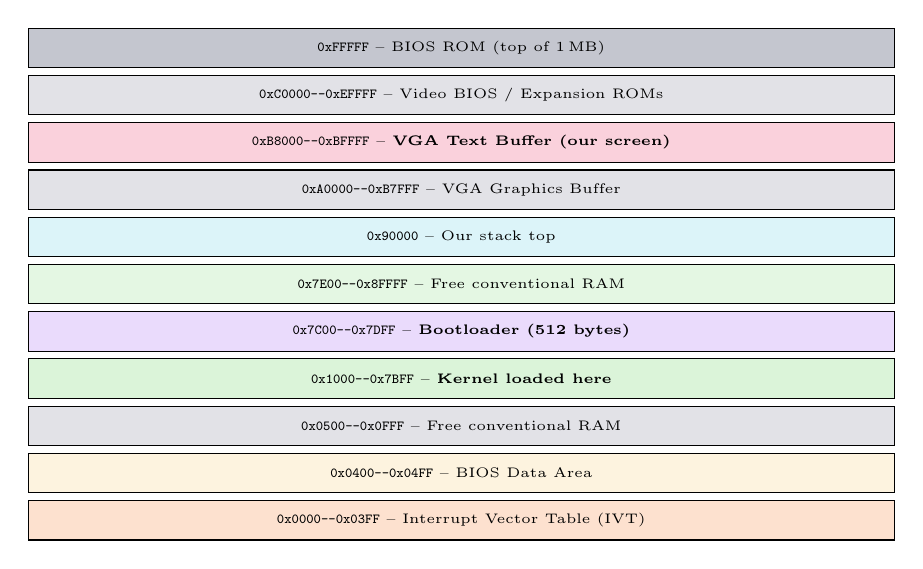
\begin{tikzpicture}[
      box/.style={rectangle,draw,minimum width=11cm,
                  minimum height=0.5cm,align=center,font=\tiny}]
    \node[box,fill=codegray!40]   at(0,6.0){\texttt{0xFFFFF} -- BIOS ROM (top of 1\,MB)};
    \node[box,fill=codegray!20]   at(0,5.4){\texttt{0xC0000--0xEFFFF} -- Video BIOS / Expansion ROMs};
    \node[box,fill=alertred!40]   at(0,4.8){\texttt{0xB8000--0xBFFFF} -- \textbf{VGA Text Buffer (our screen)}};
    \node[box,fill=codegray!20]   at(0,4.2){\texttt{0xA0000--0xB7FFF} -- VGA Graphics Buffer};
    \node[box,fill=codeblue!30]   at(0,3.6){\texttt{0x90000} -- Our stack top};
    \node[box,fill=codegreen!30]  at(0,3.0){\texttt{0x7E00--0x8FFFF} -- Free conventional RAM};
    \node[box,fill=codepurple!40] at(0,2.4){\texttt{0x7C00--0x7DFF} -- \textbf{Bootloader (512 bytes)}};
    \node[box,fill=codegreen!40]  at(0,1.8){\texttt{0x1000--0x7BFF} -- \textbf{Kernel loaded here}};
    \node[box,fill=codegray!20]   at(0,1.2){\texttt{0x0500--0x0FFF} -- Free conventional RAM};
    \node[box,fill=codeyellow!40] at(0,0.6){\texttt{0x0400--0x04FF} -- BIOS Data Area};
    \node[box,fill=codeorange!40] at(0,0.0){\texttt{0x0000--0x03FF} -- Interrupt Vector Table (IVT)};
  \end{tikzpicture}
  \end{center}
\end{frame}

%% ════════════════════════════════════════════════════════════════════════════
\section{What We Built and What Comes Next}
%% ════════════════════════════════════════════════════════════════════════════

\begin{frame}{What We Built --- Summary}
  \begin{columns}[T]
    \column{0.5\textwidth}
    \textbf{Bootloader (\texttt{boot/bootloader.asm})}
    \begin{itemize}
      \item 16-bit real mode setup
      \item BIOS disk read (int 0x13)
      \item A20 enable
      \item GDT construction
      \item Protected mode switch
    \end{itemize}
    \vspace{8pt}
    \textbf{Linker script (\texttt{linker.ld})}
    \begin{itemize}
      \item Places kernel at 0x1000
      \item Flat binary output
    \end{itemize}
    \column{0.5\textwidth}
    \textbf{Kernel entry (\texttt{kernel/kernel\_entry.asm})}
    \begin{itemize}
      \item Sets up stack
      \item Calls \texttt{kernel\_main()}
      \item Safe halt
    \end{itemize}
    \vspace{8pt}
    \textbf{Kernel module (\texttt{kernel/screen.c + screen.h})}
    \begin{itemize}
      \item Terminal API: \texttt{print()}, \texttt{put\_char()}, \texttt{set\_color()}
      \item Cursor tracking + newline handling
      \item Automatic scrolling at row overflow
      \item Screen clear with current colour attribute
    \end{itemize}
  \end{columns}
\end{frame}

\begin{frame}{Core Concepts Learned}
  \begin{tabular}{ll}
    \toprule
    \textbf{Concept} & \textbf{What you now understand}\\
    \midrule
    BIOS boot process    & Power-on to bootloader in 8 steps\\
    Real vs Protected Mode& 16-bit/1 MB vs 32-bit/4 GB\\
    Segmentation / GDT   & How CPU enforces memory layout in PM\\
    Flat memory model    & base=0, limit=4 GB for simplicity\\
    VGA text buffer      & Direct memory-mapped hardware access\\
    Linker scripts       & How addresses are assigned at link time\\
    Cross-compilation    & Compiling for a different target architecture\\
    Triple fault         & CPU reset caused by unhandled exceptions\\
    Interrupt safety     & Why \texttt{cli} is mandatory in PM without IDT\\
    Disk images          & How \texttt{dd} builds raw sector-by-sector images\\
    \bottomrule
  \end{tabular}
\end{frame}

\begin{frame}{Next Steps --- Build the Rest of the OS}
  \begin{columns}
    \column{0.5\textwidth}
    \textbf{Immediate next:}
    \begin{enumerate}
      \item \textbf{IDT} -- Interrupt Descriptor Table\\
        Handle CPU exceptions properly
      \item \textbf{PIC} -- 8259 Programmable Interrupt Controller\\
        Enable hardware interrupts safely
      \item \textbf{Keyboard driver}\\
        Read port 0x60, map scancodes
      \item \textbf{Shell}\\
        Accept typed commands
    \end{enumerate}
    \column{0.5\textwidth}
    \textbf{Medium term:}
    \begin{enumerate}
      \item \textbf{Physical Memory Manager}\\
        Track free/used RAM pages
      \item \textbf{Virtual Memory / Paging}\\
        Isolate processes from kernel
      \item \textbf{Heap allocator}\\
        Implement \texttt{kmalloc}/\texttt{kfree}
      \item \textbf{VFS + FAT filesystem}\\
        Read/write files
      \item \textbf{ELF loader}\\
        Run user-space programs
    \end{enumerate}
  \end{columns}
\end{frame}

\begin{frame}{Further Reading}
  \begin{itemize}
    \item \textbf{OSDev Wiki} --- \url{https://wiki.osdev.org} \\
      The definitive community resource for OS development
    \item \textbf{Intel Software Developer Manuals} --- \url{https://www.intel.com/content/www/us/en/developer/articles/technical/intel-sdm.html}\\
      Official CPU architecture reference (free PDF)
    \item \textbf{``Writing a Simple Operating System from Scratch''} --- Nick Blundell (free PDF)\\
      Step-by-step guide covering many topics we explored
    \item \textbf{``OS: Three Easy Pieces''} --- Arpaci-Dusseau (free online)\\
      \url{https://ostep.org} --- Best OS theory textbook
    \item \textbf{NASM Manual} --- \url{https://nasm.us/doc}\\
      Complete assembler documentation
  \end{itemize}
  \vspace{8pt}
  \begin{center}
    \Large \textbf{You just built an OS from scratch.}\\[4pt]
    \normalsize That puts you in a very small group of programmers.
  \end{center}
\end{frame}

\begin{frame}[plain]
  \begin{center}
    \vspace{1cm}
    {\Huge \textbf{MyOS v0.1}}\\[0.5cm]
    {\large Running in 32-bit Protected Mode}\\[1cm]
    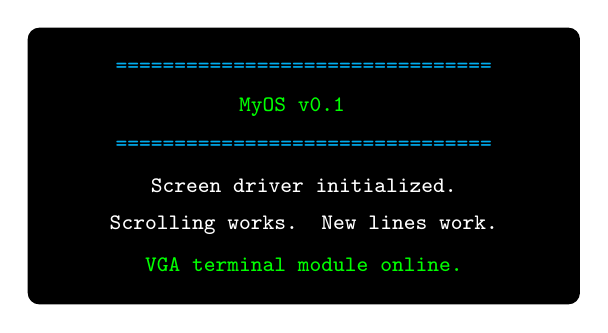
\begin{tikzpicture}
      \draw[fill=black,rounded corners=4pt] (0,0) rectangle (7,3.5);
      \node[font=\ttfamily\footnotesize,color=cyan]    at(3.5,3.0){================================};
      \node[font=\ttfamily\footnotesize,color=green]   at(3.5,2.5){\quad\quad\quad MyOS v0.1\quad\quad\quad\quad\quad};
      \node[font=\ttfamily\footnotesize,color=cyan]    at(3.5,2.0){================================};
      \node[font=\ttfamily\footnotesize,color=white]   at(3.5,1.5){Screen driver initialized.};
      \node[font=\ttfamily\footnotesize,color=white]   at(3.5,1.0){Scrolling works. New lines work.};
      \node[font=\ttfamily\footnotesize,color=green]   at(3.5,0.5){VGA terminal module online.};
    \end{tikzpicture}\\[0.8cm]
    {\large From zero to OS in one session.}
  \end{center}
\end{frame}

\end{document}
